\begin{figure}[H]
	\centerline{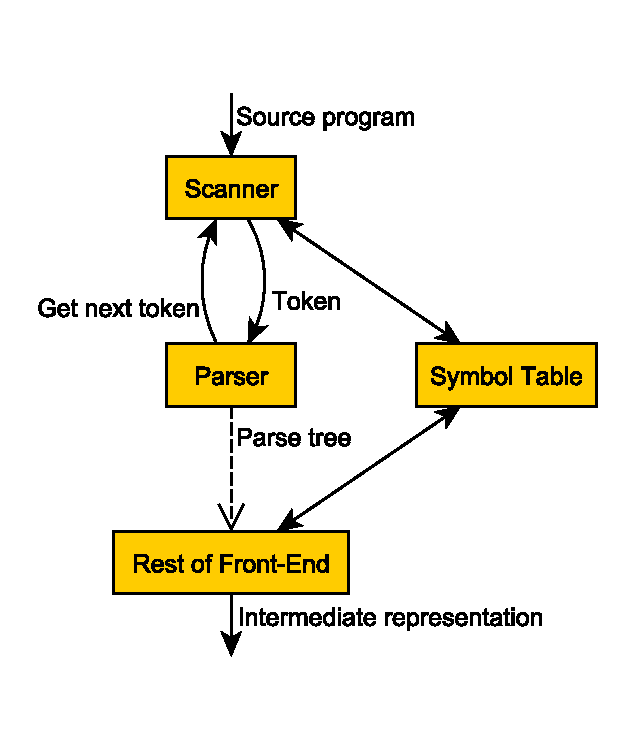
\includegraphics[width=0.6\textwidth]{img/13.pdf}}
\end{figure}

Tokens are terminal symbols in the grammar for the source language.
Lexeme is a string of characters in the source program treated as a lexical unit.
Pattern is a representation of the set of lexemes associated with a token.

\section{Role of a Scanner}
Upon receiving a ``get next token'' command from the parser, the scanner reads input characters until it can identify a token.
Scanner simplifies the job of the parser:
\begin{itemize}
	\item it discards as many irrelevant details as possible;
	\item parser rules are only concerned with tokens, not with lexemes.
\end{itemize}
Also, scanner improves compiler efficiency.

\section{Regular Definitions}
A regular definition is a sequence of definitions:
$$
	d_1 \to r_1; d_2 \to r_2; \ldots; d_n \to r_n
$$
Each $d_i$ is a distinct name (token); each $r_i$ is a regular expression, over $\Sigma \cup \left\{d_1, \ldots, d_{i-1}\right\}$ representing a pattern.

The task of constructing a lexical-analyser is simple enough to be automated.
A lexical-analyser generator transforms the specification of a scanner into a program implementing a finite automaton accepting the specified lexemes.